\chapter{SİN\texorpdfstring{\textsuperscript{3}}{3} TABANLI İLERİ BESLEME KOMPANZASYONU VE KAPALI ÇEVRİM ANALİZİ}
\label{chap:sin3}

Nötr anahtar susturma yöntemi ters akım dolaşımını azaltmayı hedeflerken akımı süreksiz iletime zorlamakta ve özellikle düşük mertebeli harmonikleri büyütmektedir. Bölüm~\ref{chap:anahtarlama} altındaki senaryo kayıtları, çıkış akımı THD değerinin klasik yöntemdeki \%2,14 düzeyinden susturma sonrasında \%46,35 düzeyine çıktığını; Sin\textsuperscript{3} kompanzasyonu eklendiğinde ise \%7,79'a gerilediğini göstermiştir. Bölümün amacı bu iyileşmenin arkasındaki matematiksel yapıyı kurmak, kompanzasyon katsayılarını doğru trigonometrik özdeşlikle ve doğrulanmış parametre setiyle yeniden hesaplamak ve kapalı çevrim ile kararlılık incelemesinin yöntemini vermektir.

\section{Sin\texorpdfstring{\textsuperscript{3}}{3} Bileşeninin Matematiksel Tanımı}

Zaman $t$, şebeke temel açısal frekansı $\omega_0$, PLL faz başlangıcı/ofseti $\phi$ ve boyutsuz elektriksel açı $\theta=\omega_0t+\phi$ ile gösterilsin. Kullanılan trigonometrik özdeşlik
\begin{equation}
  \sin^3\theta=\frac{3}{4}\sin\theta-\frac{1}{4}\sin(3\theta)
  \label{eq:sin3-acilimi}
\end{equation}
biçimindedir. Eşitlik~\eqref{eq:sin3-acilimi} uyarınca $\sin^3\theta$ terimi yalnız üçüncü harmonikten oluşmaz; temel bileşen ile ters işaretli üçüncü harmonik bileşenini sabit bir oranla birlikte taşır. Boyutsuz Sin\textsuperscript{3} ileri besleme komutu $u_{\mathrm{ff},\sin^3}(\theta)$, temel bileşen kazanç katsayısı $K_1$ ve küp teriminin kazanç katsayısı $K_3$ ile
\begin{equation}
  u_{\mathrm{ff},\sin^3}(\theta)=K_1\sin\theta+K_3\sin^3\theta
  \label{eq:sin3-genel-komut}
\end{equation}
olarak tanımlandığında Eşitlik~\eqref{eq:sin3-acilimi} kullanılarak
\begin{equation}
  u_{\mathrm{ff},\sin^3}(\theta)
  =\left(K_1+\frac{3K_3}{4}\right)\sin\theta-\frac{K_3}{4}\sin(3\theta)
  =A_1\sin\theta+A_3\sin(3\theta)
  \label{eq:sin3-esdeger-katsayilar}
\end{equation}
elde edilir. Eşitlik~\eqref{eq:sin3-genel-komut} ile Eşitlik~\eqref{eq:sin3-esdeger-katsayilar} arasındaki dönüşümde $A_1=K_1+3K_3/4$ temel sinüs katsayısını, $A_3=-K_3/4$ ise doğrudan üçüncü harmonik katsayısını gösterir. Yazılımda doğrudan $\sin(3\theta)$ kullanılması ile $\sin^3\theta$ kullanılması aynı işlem değildir; gerçek uygulama kodu geldiğinde kullanılan gösterim, katsayı ve işaret Eşitlik~\eqref{eq:sin3-esdeger-katsayilar} üzerinden kilitlenecektir.

\section{Basitleştirilmiş Türetimlerin Geçerlilik Sınırı}

Kompanzasyon katsayılarının tek bir cebirsel iptal koşulundan (örneğin sabit bir $K_1/K_3$ oranından) türetilmesi cazip görünse de anahtarlamalı dönüştürücüde geçerli değildir. Bunun üç nedeni vardır. Birincisi, belirli bir çalışma noktasında gözlenen temel ve üçüncü harmonik genliklerinin oranı, girişten bağımsız bir sistem transfer fonksiyonu değildir; yalnız o dalga biçimini ve o çalışma noktasını tarif eder. İkincisi, anahtarlamalı, doğrusal olmayan veya periyodik zamanla değişen bir sistemde süperpozisyon kanıtlanmadan uygulanamaz; giriş dalga biçimi değiştirildiğinde aynı skaler oranın yeniden kullanılması örtük bir doğrusallık varsayımıdır. Üçüncüsü, komutun frekans içeriği ile dönüştürücünün çıkış akımı aynı büyüklük değildir; çıkıştaki harmonik iptal koşulu, bitki dinamiği ve harmonikler arası bağlaşım bilinmeden yalnız trigonometrik özdeşlikten çıkarılamaz.

Periyodik zamanla değişen sistemin doğru genel çerçevesi harmonik transfer fonksiyonudur. Kesilmiş harmonik giriş ve çıkış vektörleri $\mathbf{U}(s)$ ile $\mathbf{I}(s)$, harmonik transfer matrisi $\mathbf{G}_{\mathrm{H}}(s)$, matrisin $(k,n)$ elemanı $G_{k,n}(s)$ ve kesme mertebesi $N_h$ ile gösterildiğinde
\begin{equation}
  \mathbf{I}(s)=\mathbf{G}_{\mathrm{H}}(s)\mathbf{U}(s),
  \qquad
  I_k(s)=\sum_{n=-N_h}^{N_h}G_{k,n}(s)U_n(s)
  \label{eq:htf-matris-iliskisi}
\end{equation}
yazılır \citep{Wereley1991,Liao2022}. Eşitlik~\eqref{eq:htf-matris-iliskisi}, tek bir giriş harmoniğinin birden fazla çıkış harmoniğine bağlaşabileceğini gösterir. Geçerli bir HTF modeli için çalışma noktası, frekans taraması, $N_h$ ve kesme hatası birlikte belirtilmelidir. Kompanzasyon katsayıları bu çerçevede ya periyodik çalışma noktası çevresinde doğrusallaştırılmış model üzerinden ya da küçük işaretli temel ve üçüncü harmonik enjeksiyon ölçümleriyle belirlenmelidir; katsayıların çalışma noktasına bağlılığı Kesim~\ref{sec:sin3-yeniden-tarama} altında sayısal olarak da gösterilmektedir.

Kompanzasyonun hedefi, akımın ölçülen üçüncü harmonik fazına ters yönde bir modülasyon bileşeni üretirken temel akım genliğini korumaktır. Uygulama kazancı yalnız THD eniyilemesiyle seçilmemeli; modülasyon doygunluğu, DA bara kullanımı, akım RMS değeri, kontrol eforu ve düşük güçten orta güce geçişte süreklilik koşulları birlikte değerlendirilmelidir. Üçüncü harmonik enjeksiyonunun modülasyon kullanımını değiştirebildiği bilinse de buradaki amaç klasik üçüncü harmonik PWM ile DA bara kullanımını artırmak değil, nötr susturmanın oluşturduğu akım zarfı bozulmasını azaltmaktır \citep{Holmes2003}.

\eksikistek{Gerçek Sin\textsuperscript{3} kodu ve harmonik bağlaşım ölçümü}{(1) Uygulamadaki ileri besleme ifadesinin $K_1\sin\theta+K_3\sin^3\theta$ mı yoksa $K_1\sin\theta+K_3\sin(3\theta)$ mı olduğunu; işaret, normalizasyon, birim, doyum ve etkinleştirme koşullarıyla birlikte gösteren kaynak kodu istiyoruz (istek listesi R07). (2) Temel ve üçüncü harmonik giriş--çıkış bağlaşımını belirlemek için model doğrusallaştırması veya küçük işaretli harmonik enjeksiyon taraması istiyoruz; Eşitlik~\eqref{eq:htf-matris-iliskisi} bu veriler olmadan sayısallaştırılamaz.}

\section{Düşük Güçte Harmonik Oluşum Mekanizması}

Şekil~\ref{fig:senkron-buck-esdeger} altında verilen iki-buck eşdeğeri, pozitif ve negatif alternansların aynı fiziksel mekanizmayla incelenmesini sağlar. Pozitif alternansta etkin yarım bara gerilimi $V_h$, anık şebeke gerilimi $v_g(\theta)>0$, anahtarlama periyodu $T_s$, boyutsuz görev oranı $d(\theta)\in[0,1]$ ve eşdeğer endüktans $L$ olarak tanımlansın. İdeal anahtarlama-periyodu modeli ve periyot boyunca yaklaşık sabit gerilim kabulü altında anahtar iletim süresindeki akım tepe değeri $I_{\mathrm{pk}}(\theta)$
\begin{equation}
  I_{\mathrm{pk}}(\theta)=\frac{V_h-v_g(\theta)}{L}\,d(\theta)T_s
  \label{eq:dcm-tepe-akimi}
\end{equation}
olur. Eşitlik~\eqref{eq:dcm-tepe-akimi}, iletim başlangıcında akımın sıfır olduğu DCM darbesi içindir. Anahtar kesime girdiğinde akım $-v_g/L$ eğimiyle sıfıra düşerse, gerçek boşalma süresinin $T_s$'ye oranı olan boyutsuz $\delta(\theta)$
\begin{equation}
  \delta(\theta)=\left(\frac{V_h}{v_g(\theta)}-1\right)d(\theta)
  \label{eq:dcm-bosalma-suresi}
\end{equation}
olarak bulunur. Eşitlik~\eqref{eq:dcm-bosalma-suresi}, yalnızca $v_g(\theta)>0$ ve akımın aynı periyotta sıfıra ulaştığı aralıkta geçerlidir. Üçgensel akım darbesinin bir anahtarlama periyodundaki ortalaması $\bar i_L(\theta)$
\begin{equation}
  \bar i_L(\theta)=\frac{1}{2}I_{\mathrm{pk}}(\theta)\,[d(\theta)+\delta(\theta)]
  =\frac{T_sV_h}{2L}\frac{V_h-v_g(\theta)}{v_g(\theta)}d^2(\theta)
  \label{eq:dcm-ortalama-akim}
\end{equation}
ifadesini verir \citep{Erickson2001,Chen2010}. Eşitlik~\eqref{eq:dcm-ortalama-akim}, Eşitlik~\eqref{eq:dcm-tepe-akimi} ile Eşitlik~\eqref{eq:dcm-bosalma-suresi} kullanılarak üçgen alanından elde edilmiştir. Sinüzoidal görev oranının tepe katsayısı $d_m$ ve şebeke geriliminin tepe değeri $V_m$ olmak üzere $d(\theta)=d_m\sin\theta$ ve $v_g(\theta)=V_m\sin\theta$ kabulü altında pozitif alternans zarfı
\begin{equation}
  \bar i_L(\theta)=\frac{T_sV_hd_m^2}{2LV_m}\sin\theta\,[V_h-V_m\sin\theta],
  \qquad 0<\theta<\pi
  \label{eq:dcm-sinus-zarfi}
\end{equation}
biçimine dönüşür. Eşitlik~\eqref{eq:dcm-sinus-zarfi}, görev oranı sinüzoidal olsa bile ortalama akımın saf sinüs kalmadığını doğrudan göstermektedir: zarf, $\sin\theta$ ile $[V_h-V_m\sin\theta]$ çarpımından oluştuğu için sıfır geçişlerinde sinüsten hızlı yükselir ve alternans ortasında çöker. Düşük güçte çalışma noktasına bağlı akım harmoniklerinin büyüyebildiği, saha ölçümü ile zamanla değişen modeller üzerinden de raporlanmıştır \citep{Chicco2009,Du2013}.

DCM koşulu darbenin aynı anahtarlama periyodunda sona ermesini gerektirir:
\begin{equation}
  d(\theta)+\delta(\theta)\leq 1
  \quad\Longrightarrow\quad
  d(\theta)\leq d_{\mathrm{krit}}(\theta)=\frac{v_g(\theta)}{V_h}.
  \label{eq:dcm-kritik-gorev}
\end{equation}
Eşitlik~\eqref{eq:dcm-kritik-gorev} içindeki kritik görev oranı faz açısına ve gerilim oranına bağlıdır; tek bir evrensel sayı değildir. Doğrulanmış parametre setinde ($V_h=\SI{215.75}{\volt}$, $V_m=\SI{169.4}{\volt}$) tepe değeri $V_m/V_h\simeq0{,}785$'tir ve Kesim~\ref{sec:sin3-yeniden-tarama} altındaki sayısal tarama, $d_m$ bu sınırı aştığında alternans ortasında CCM'ye geçildiğini doğrulamaktadır. Sıfır geçişte $v_g\rightarrow0$ olduğundan ideal ifadenin tek başına kullanılması uygun değildir; ölü zaman, minimum darbe ve sonlu akım eşiği ayrıca uygulanmalıdır.

DCM zarfı ile sürekli iletim modeli ortak bir görev oranı üzerinden birleştirilebilir. Temel ve üçüncü harmonik görev katsayıları $D_1$ ve $D_3$ kullanılarak
\begin{equation}
  d(\theta)=D_1\sin\theta+D_3\sin^3\theta
  \label{eq:ccm-gorev-harmonik}
\end{equation}
yazılsın; Eşitlik~\eqref{eq:ccm-gorev-harmonik} içindeki $D_1$ ve $D_3$, Eşitlik~\eqref{eq:sin3-esdeger-katsayilar} altındaki $K_1$ ile $K_3$'e uygulama ölçeklemesi sonrası karşılık gelen görev katsayılarıdır. Pozitif alternansta kayıpsız CCM ortalama diferansiyel denklemi
\begin{equation}
  L\frac{\mathrm{d}\bar i_{L,\mathrm{CCM}}}{\mathrm{d}t}
  =V_h d(\theta)-V_m\sin\theta
  \label{eq:ccm-diferansiyel}
\end{equation}
biçimindedir \citep{Erickson2001,Mohan2003}. Eşitlik~\eqref{eq:ccm-diferansiyel}, $\theta=\omega_0t+\phi$ bağı ve Eşitlik~\eqref{eq:ccm-gorev-harmonik} kullanılarak integre edildiğinde
\begin{equation}
  \bar i_{L,\mathrm{CCM}}(\theta)
  = I_0+\frac{V_m-V_hD_1}{\omega_0L}\cos\theta
  -\frac{V_hD_3}{3\omega_0L}\cos(3\theta)
  \label{eq:ccm-akim-cozumu}
\end{equation}
elde edilir; burada $\sin^3\theta$ önce Eşitlik~\eqref{eq:sin3-acilimi} ile harmonik bileşenlerine ayrılmıştır ve $I_0$, DCM--CCM geçişinde akım sürekliliğinden belirlenen integrasyon sabitidir. Anahtarlama-periyodu ortalama akımının parçalı modeli
\begin{equation}
  \bar i_L(\theta)=
  \begin{cases}
    \bar i_{L,\mathrm{DCM}}(\theta), & d(\theta)<d_{\mathrm{krit}}(\theta),\\
    \bar i_{L,\mathrm{CCM}}(\theta), & d(\theta)\geq d_{\mathrm{krit}}(\theta)
  \end{cases}
  \label{eq:dcm-ccm-parcali-model}
\end{equation}
ile ifade edilir. Tam periyot şebeke akımı $i_g(\theta)$ yarım dalga tek simetrisine sahipse $n$'inci sinüs Fourier katsayısı
\begin{equation}
  B_n=\frac{1}{\pi}\int_0^{2\pi}i_g(\theta)\sin(n\theta)\,\mathrm{d}\theta,
  \qquad n=1,2,\ldots
  \label{eq:akim-fourier-katsayisi}
\end{equation}
olarak hesaplanır \citep{Oppenheim1997}. Eşitlik~\eqref{eq:akim-fourier-katsayisi} içindeki $B_1$ ve $B_3$ sırasıyla temel ve üçüncü harmonik sinüs katsayılarını verir; yarım dalga simetrisi sağlanmazsa DA ve kosinüs katsayıları da ayrıca hesaplanmalıdır.

\section{Katsayıların Doğru Özdeşlikle Yeniden Hesabı}
\label{sec:sin3-yeniden-tarama}

Eşitlik~\eqref{eq:dcm-tepe-akimi}--\eqref{eq:dcm-ccm-parcali-model} ile kurulan parçalı model, kompanzasyon katsayılarının sayısal olarak taranmasına olanak tanır. Tarama 01.09.2026 tarihli MATLAB koşusuyla, doğrulanmış parametre seti ($V_{\mathrm{dc}}=\SI{431.5}{\volt}$, $V_h=\SI{215.75}{\volt}$, $V_m=\SI{169.4}{\volt}$, $f_0=\SI{50}{\hertz}$, $f_s=\SI{10}{\kilo\hertz}$, $L=L_1=\SI{600}{\micro\henry}$) üzerinde yapılmıştır. Model, nötr anahtarı susturulmuş faz kolunu anahtarlama periyodu bazında parçalı doğrusal çözmekte; susturma nedeniyle akım tabanı sıfırda kesilmekte ve DCM--CCM geçişleri periyotlar arası başlangıç akımıyla doğal olarak oluşmaktadır. Kanıt sınırı açıktır: bu, Tablo~\ref{tab:model-katmanlari} içindeki analitik/ortalama katmandır; ölü zaman, denetleyici, $C_f$--$L_2$ dinamiği ve kayıplar içermez, verim sonucu üretmez.

Üç bulgu öne çıkmaktadır. Birincisi, saf sinüzoidal görev oranıyla ($D_3=0$) süreksiz iletimdeki üçüncü harmonik oranı $d_m=0{,}1$--$0{,}7$ aralığında sabit \%39,96 çıkmaktadır; Tablo~\ref{tab:dcm-saf-sinus-harmonikleri} bu taramayı vermektedir. Oranın $d_m$'den bağımsızlığı, Eşitlik~\eqref{eq:dcm-sinus-zarfi} zarfının şeklinin $d_m^2$ ölçeklemesinden bağımsız olmasının doğrudan sonucudur. $d_m=0{,}8$ satırında oran değişmekte ve akım hızla büyümektedir; bu, $d_{\mathrm{krit}}$ tepe değerinin ($\simeq0{,}785$) aşılıp alternans ortasında CCM'ye geçilmesinin göstergesidir ve ideal tam-DCM modelinin geçerlilik sınırını işaretler.

\begin{table}[htbp]
  \centering
  \caption{Saf sinüzoidal görev oranı için parçalı DCM/CCM modelinden hesaplanan harmonik genlikler (01.09.2026 koşusu).}
  \label{tab:dcm-saf-sinus-harmonikleri}
  \small
  \begin{tabular}{S[table-format=1.1] S[table-format=1.4] S[table-format=1.4] S[table-format=1.4] S[table-format=1.4] S[table-format=2.2]}
    \toprule
    {$d_m$} & {$I_1$ (A)} & {$I_3$ (A)} & {$I_5$ (A)} & {$I_7$ (A)} & {$100I_3/I_1$} \\
    \midrule
    0.1 & 0.0764 & 0.0305 & 0.0044 & 0.0015 & 39.96 \\
    0.2 & 0.3055 & 0.1221 & 0.0174 & 0.0058 & 39.96 \\
    0.3 & 0.6874 & 0.2747 & 0.0392 & 0.0131 & 39.96 \\
    0.4 & 1.2220 & 0.4884 & 0.0698 & 0.0233 & 39.96 \\
    0.5 & 1.9093 & 0.7631 & 0.1090 & 0.0363 & 39.96 \\
    0.6 & 2.7494 & 1.0988 & 0.1570 & 0.0523 & 39.96 \\
    0.7 & 3.7423 & 1.4956 & 0.2137 & 0.0712 & 39.96 \\
    \bottomrule
  \end{tabular}
\end{table}

İkincisi, önceki katsayı taramalarında öne çıkan aday çiftler doğrulanmış parametre setine taşınamamaktadır. $(D_1,D_3)$ için $(0{,}45,\ 0{,}37)$, $(0{,}44,\ 0{,}38)$ ve $(0{,}41,\ 0{,}41)$ noktaları bu sette $I_1\simeq8{,}5$--\SI{9.2}{\ampere} temel akım (gerçek düşük güç çalışma noktasının yaklaşık dört katı), $I_3/I_1\simeq\%50$ ve $\mathrm{THD}\simeq\%68$ üretmektedir. Aynı adayların daha önce \%1--2 düzeyinde üçüncü harmonik oranıyla raporlanmış olması çelişki değildir; katsayıların gerilim oranına, endüktansa ve akım seviyesine bağlı olduğunu, tek bir $(D_1,D_3)$ çiftinin bütün çalışma noktalarına genellenemeyeceğini gösterir. Bulgu, üç fazlı fiziksel modeldeki bağımsız yeniden koşunun (Kesim~\ref{sec:sin3-guc-karsilastirma}) tarihsel THD iyileşmesini üretememesiyle de tutarlıdır.

Üçüncüsü, aynı tarama gerçek düşük güç çalışma noktası için düzeltilmiş bir aday vermektedir. $I_{\mathrm{rms}}$ değeri deney kayıtlarındaki \SI{2.26}{\ampere} düzeyiyle uyumlu ($2{,}0$--\SI{2.6}{\ampere}) tutulup görev oranı kırpılması dışlandığında en iyi nokta
\begin{equation}
  (D_1, D_3)=(0{,}34,\ 0{,}40)
  \;\Longrightarrow\;
  \frac{I_3}{I_1}=\%0{,}15,\quad \mathrm{THD}=\%4{,}72,\quad I_{\mathrm{rms}}=\SI{2.02}{\ampere},\quad d_{\max}=0{,}74
  \label{eq:sin3-duzeltilmis-optimum}
\end{equation}
olarak bulunmuştur; Eşitlik~\eqref{eq:sin3-esdeger-katsayilar} ile doğrudan-harmonik eşdeğeri $(A_1,A_3)=(0{,}64,\ -0{,}10)$'dur. Şekil~\ref{fig:sin3-yeniden-tarama}, katsayı düzlemindeki üçüncü harmonik oranını, uygun akım bölgesini ve en iyi noktadaki akım zarfının saf sinüs görev oranına göre düzelmesini birlikte göstermektedir. Kompanzasyonlu zarfta kalan \%4,7'lik THD, ağırlıkla beşinci ve yedinci harmoniklerden gelmektedir; Sin\textsuperscript{3} terimi yapısı gereği yalnız temel ve üçüncü harmoniği şekillendirdiğinden bu kalıntı, yöntemin yapısal sınırıdır.

\begin{figure}[htbp]
  \centering
  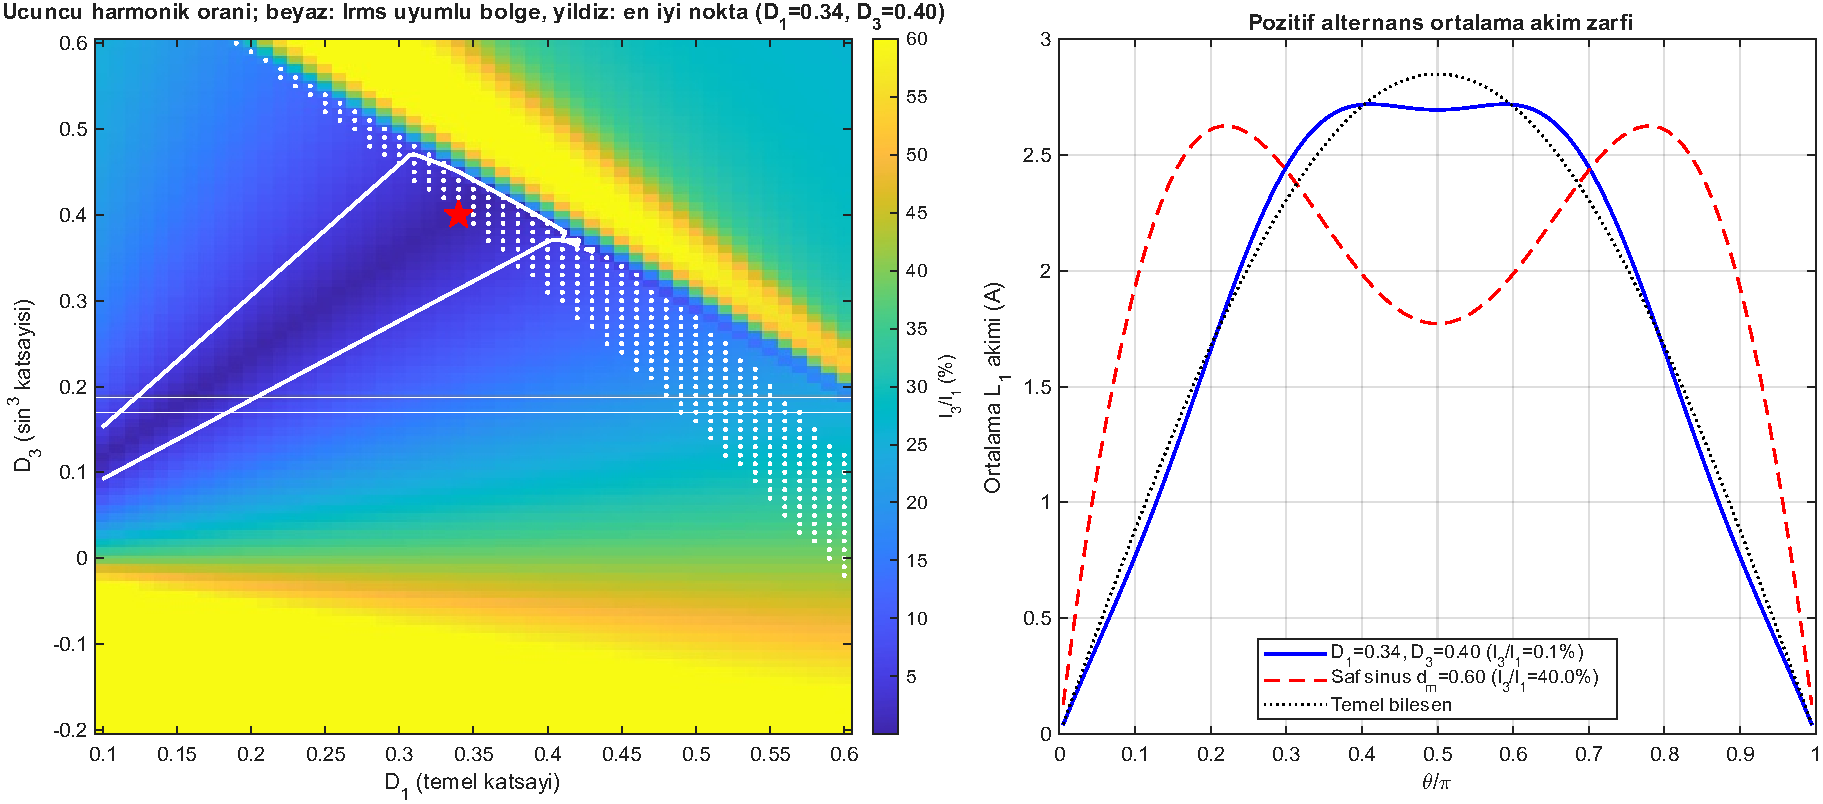
\includegraphics[width=\textwidth]{../tez-matlab-simulink/results/sin3_rescan_20260901/sin3_katsayi_taramasi_20260901.pdf}
  \caption{$(D_1,D_3)$ katsayı düzleminde üçüncü harmonik oranı (sol; beyaz noktalar \SI{2.0}{}--\SI{2.6}{\ampere} RMS bölgesini, yıldız en iyi noktayı gösterir) ve en iyi nokta ile saf sinüs görev oranının ortalama akım zarfı karşılaştırması (sağ). Parçalı DCM/CCM analitik modeli, 01.09.2026 koşusu.}
  \label{fig:sin3-yeniden-tarama}
\end{figure}

Eşitlik~\eqref{eq:sin3-duzeltilmis-optimum} ile verilen çift, uygulanacak nihai kazanç değil, doğrulanmış parametre setiyle tutarlı ilk analitik adaydır. Nihai seçim; gerçek koddaki gösterim (Eşitlik~\eqref{eq:sin3-esdeger-katsayilar} ayrımı), anahtarlamalı model, ölü zaman ve kapalı çevrim etkileşimi doğrulandıktan sonra yapılacaktır.

\section{Önerilen Yapı ve İleri Besleme Mekanizması}

İleri besleme yolunun fiziksel işlevi, evirici tarafındaki eşdeğer kaynak gerilimini şebeke gerilimine yaklaştırmaktır. PLL şebekeye kilitlendikten sonra, akım komutu uygulanmadan önce, evirici çıkışı ile şebeke eşpotansiyel ise seri $Z_1+Z_2$ filtre ve şebeke empedansından akan akım sıfıra yaklaşır; Şekil~\ref{fig:eski-feedforward-etkisi} bu durumu eşdeğer kaynaklar üzerinde, Şekil~\ref{fig:eski-espotansiyel-dalga} ise gerilim dalga biçimleri ve sıfır akım kaydıyla göstermektedir. Akım referansı uygulandığında denetleyicinin üretmesi gereken ek gerilim yalnız empedans düşümünü karşılayacak küçük bir bileşendir; akım küçüldükçe bu bileşen mutlak olarak küçülür ve modeldeki küçük gerilim hataları göreli olarak daha görünür hâle gelir. İleri besleme teriminin düşük akımdaki göreli önemi bu mekanizmadan kaynaklanır.

\begin{figure}[htbp]
  \centering
  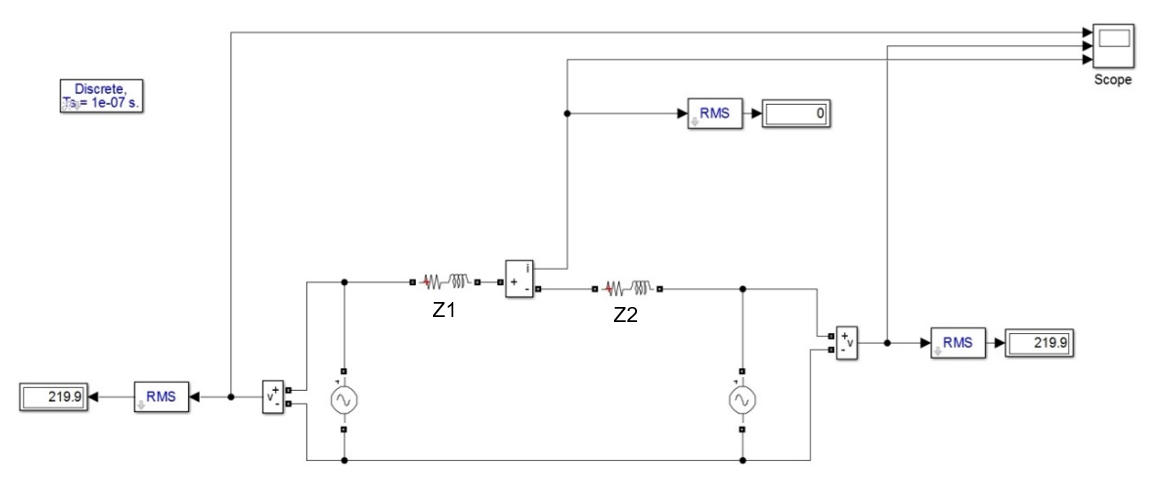
\includegraphics[width=0.96\textwidth]{sonuclar/eski_sekil_4_18_feedforward_etkisi.png}
  \caption{İleri besleme bileşeninin eşdeğer kaynaklar ve seri empedanslar üzerindeki etkisini gösteren benzetim modeli.}
  \label{fig:eski-feedforward-etkisi}
\end{figure}

\begin{figure}[htbp]
  \centering
  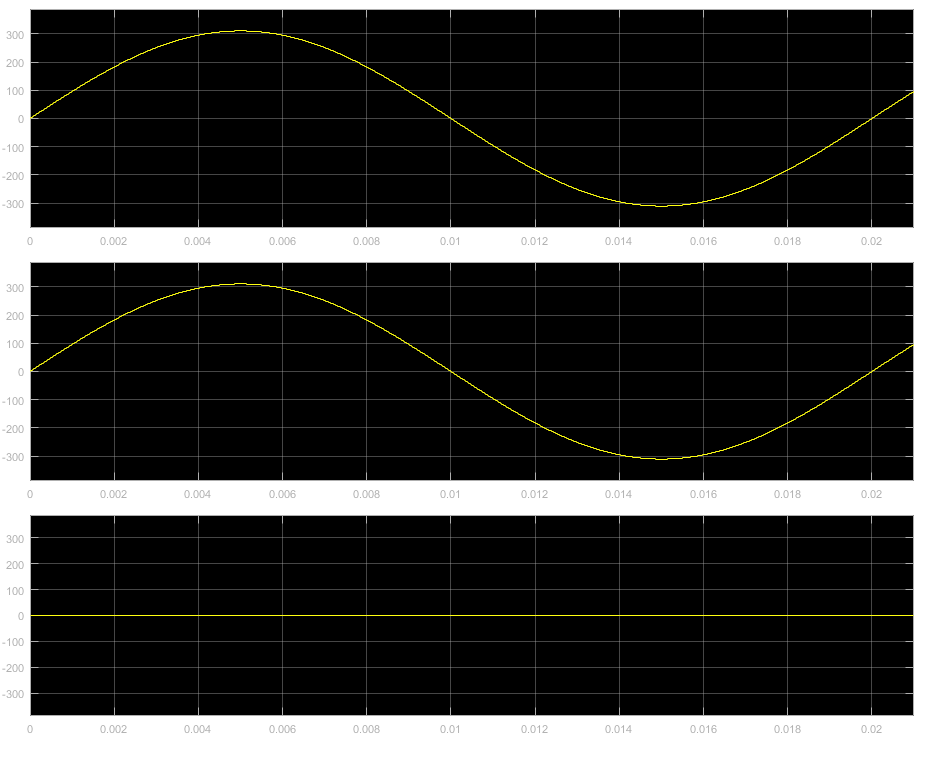
\includegraphics[width=0.90\textwidth]{sonuclar/eski_sekil_4_19_espotansiyel_dalga.png}
  \caption{Eşpotansiyel kaynakların gerilim dalga biçimleri ve kaynaklar arasındaki akımın sıfır oluşu. Kayıt, akım komutu öncesi başlangıç durumunu gösterir; kapalı çevrim izleme performansını kanıtlamaz.}
  \label{fig:eski-espotansiyel-dalga}
\end{figure}

Denetleyici devre dışı bırakılıp yalnız ileri besleme katsayısının değiştirildiği benzetim koşulu, yöntemin açık çevrim mekanizmasını ayırmak için yararlıdır; ancak kapalı çevrim performansı veya kararlılık kanıtı değildir. Şebeke gerilimi ileri beslemesi ideal durumda evirici ile şebeke gerilimini yaklaştırarak düşük akımdaki göreli gerilim hatasını azaltabilir; LCL filtre, ortak bağlantı noktası ölçümü ve dijital gecikme eklendiğinde aynı yol sanal empedans ve aktif sönümleme etkisi de oluşturabilir \citep{Lu2016}. İleri besleme yolunun etkisi bu nedenle yalnız gerilim düşümü hesabıyla sınırlandırılmamıştır. Güncel işlevsel zincir Şekil~\ref{fig:denetim-modulasyon-blok} üzerinde verilmiştir: Sin\textsuperscript{3} yolu akım denetleyicisiyle seri değil, modülasyon toplamında paralel bir ileri besleme bileşenidir ve nötr anahtar susturma kararı PWM üretiminden sonra kapı mantığında uygulanır.

\section{Kapalı Çevrim Modeli}

Faz başına gerilimden akıma LCL bitkisi $G_{vi}(s)$ Bölüm~\ref{chap:sistem} içinde Eşitlik~\eqref{eq:lcl-aktarim} ile tanımlanmıştır. PR denetleyicisi $C_i(s)$ Eşitlik~\eqref{eq:pr-denetleyici}, normalize modülasyon komutunu evirici kutup gerilimine dönüştüren PWM eşdeğer kazancı $K_{\mathrm{pwm}}$ ve toplam hesaplama--örnekleme--PWM gecikmesi $G_d(s)$ ile gösterilsin. Boyutsuz açık çevrim kazanç fonksiyonu $L(s)$
\begin{equation}
  L(s)=C_i(s)K_{\mathrm{pwm}}G_d(s)G_{vi}(s)
  \label{eq:sin3-acik-cevrim}
\end{equation}
olarak yazılır. Eşitlik~\eqref{eq:sin3-acik-cevrim} içindeki çarpanlar aynı işaret yönü ve birim sistemiyle kurulmalıdır. Toplam gecikme süresi $T_d$ olmak üzere sürekli-zaman yaklaşımında $G_d(s)=\exp(-sT_d)$ kullanılabilir; rasyonel Bode hesabında ise mertebesi belirtilmiş Padé yaklaşımı uygulanır. PR yapısının temel frekansta yüksek kazanç sağlaması sinüzoidal izleme hatasını azaltırken LCL rezonansı ek sönümleme veya uygun aktif sönümleme tasarımı gerektirir \citep{Teodorescu2006PR,Zhang2014PR}.

Referans izleme ve bozucu bastırma incelemesinde duyarlılık fonksiyonları
\begin{equation}
  S(s)=\frac{1}{1+L(s)},
  \qquad
  T(s)=\frac{L(s)}{1+L(s)}
  \label{eq:sin3-duyarlilik}
\end{equation}
biçimindedir. Eşitlik~\eqref{eq:sin3-duyarlilik} içindeki $S(s)$ duyarlılık, $T(s)$ tamamlayıcı duyarlılık fonksiyonudur. Doğrusal modelde toplama noktasına dışsal olarak eklenen $u_{\mathrm{ff},\sin^3}$ terimi Eşitlik~\eqref{eq:sin3-acik-cevrim} içindeki karakteristik paydayı tek başına değiştirmez. Gerçek uygulamada ise doygunluk, örnekleme, PLL faz hatası, anahtarlama kip değişimi ve ortak bağlantı noktası gerilimi üzerinden oluşan iç bağlaşım söz konusu ayrımı bozabilir. Şebeke gerilimi ileri beslemesinin dijital gecikmeyle birlikte LCL rezonansına sönümleme veya kararsızlaştırıcı etki verebilmesi literatürde hem model hem deneyle gösterilmiştir \citep{Lu2016,Wang2024}.

Şebeke akımı, akım referansı, Sin\textsuperscript{3} ileri besleme komutu ve şebeke geriliminin Laplace dönüşümleri sırasıyla $I_g(s)$, $I^{\ast}(s)$, $U_{\mathrm{ff},\sin^3}(s)$ ve $V_g(s)$ ile; şebeke geriliminden akıma bozucu aktarım $G_{vg}(s)$ ile gösterilsin. Harmonik kompanzasyonun doğrusal küçük işaret modeli, seçilen çalışma noktası çevresinde
\begin{equation}
  I_g(s)=T(s)I^{\ast}(s)+S(s)K_{\mathrm{pwm}}G_d(s)G_{vi}(s)U_{\mathrm{ff},\sin^3}(s)
  +S(s)G_{vg}(s)V_g(s)
  \label{eq:sin3-kapali-cevrim-girisleri}
\end{equation}
şeklinde ayrıştırılabilir; $G_{vg}(s)$'nin işareti seçilen gerilim ve akım yönlerine bağlıdır. Eşitlik~\eqref{eq:sin3-kapali-cevrim-girisleri}, Sin\textsuperscript{3} yolunun akım geri beslemesiyle seri bir denetleyici olmadığını, kapalı çevrim tarafından süzülen ayrı bir giriş olduğunu göstermektedir.

\section{Bode ve Kararlılık Marjı Analizi}

Kapalı çevrim incelemesi $L(s)$, $S(s)$ ve $T(s)$ fonksiyonlarının aynı fiziksel bitki, denetleyici ve gecikme modeliyle üretilmesine dayanır. Gerçek PR katsayıları, sönümleme ve gecikme henüz kilitlenmediğinden Şekil~\ref{fig:gecici-bode-lst} nihai kararlılık kanıtı değil, analiz zincirinin doğrulanmış filtre setiyle çalışan MATLAB çıktısıdır. Geçici parametrelerle elde edilen eğrilerin tezde tutulması yöntemi görünür kılmakta; sayısal marjların gerçek kod ve model geldiğinde aynı betikle değiştirilmesini sağlamaktadır.

\begin{figure}[htbp]
  \centering
  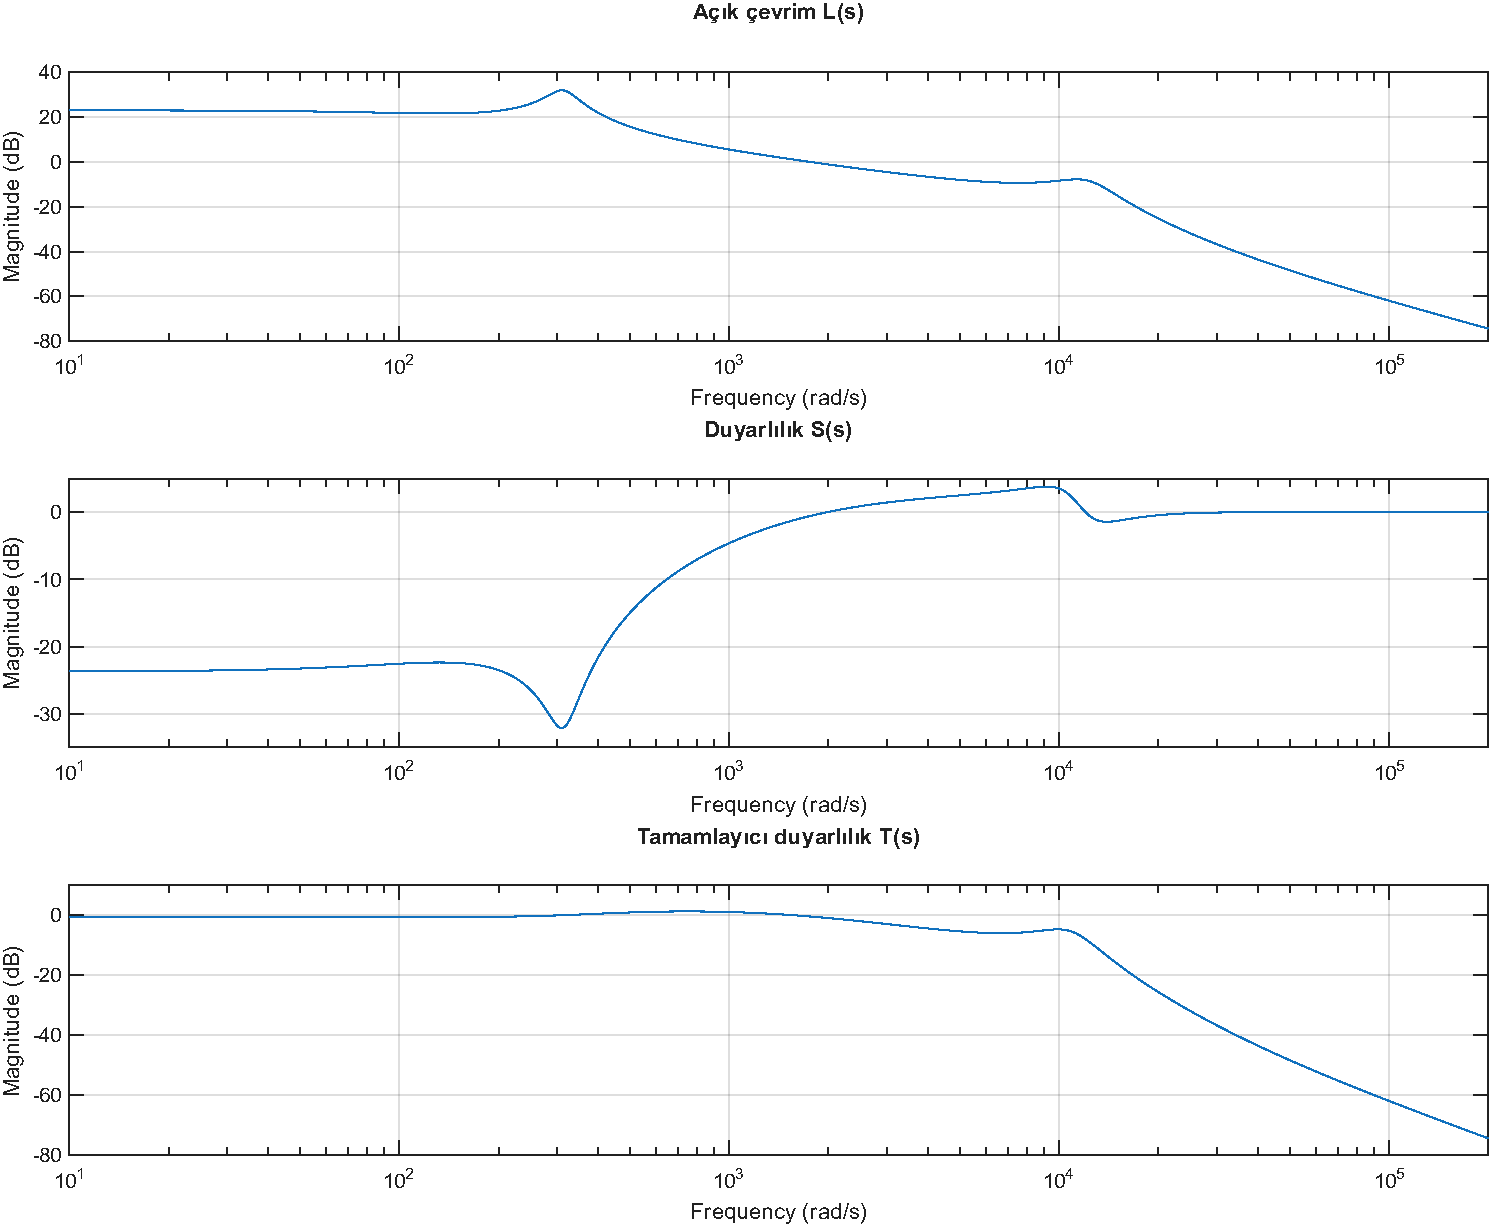
\includegraphics[width=0.96\textwidth]{../tez-matlab-simulink/results/stability/bode_LST.pdf}
  \caption{Geçici LCL--PR--gecikme modeli için MATLAB ile üretilen $L(s)$, $S(s)$ ve $T(s)$ büyüklük eğrileri; nihai parametre doğrulaması beklenmektedir.}
  \label{fig:gecici-bode-lst}
\end{figure}

Geçici modelde toplam gecikme \SI{150}{\micro\second} alınmış, kazanç marjı \SI{9.09}{\decibel} ve faz marjı $64{,}16^{\circ}$ hesaplanmıştır. Ek şebeke endüktansı $0$--\SI{2}{\milli\henry} arasında tarandığında aday model kararlı kalmış ve faz marjı $61{,}40^{\circ}$--$64{,}16^{\circ}$ aralığında değişmiştir. Sonuçlar analiz zincirinin çalıştığını gösterir; gerçek denetleyici katsayıları ve gecikme doğrulanmadan tezin nihai kararlılık marjı olarak savunulmayacaktır. Tablo~\ref{tab:sin3-kararlilik-kontrol-listesi}, incelemenin tamamlanma ölçütlerini ve mevcut durumu ayırmaktadır.

\begin{table}[htbp]
  \centering
  \caption{Kapalı çevrim kararlılık incelemesinin tamamlanma ölçütleri.}
  \label{tab:sin3-kararlilik-kontrol-listesi}
  \small
  \begin{tabularx}{\textwidth}{p{0.24\textwidth} X p{0.24\textwidth}}
    \toprule
    İnceleme & Değişkenler ve raporlanacak çıktı & Mevcut durum \\
    \midrule
    Nominal model & $L,S,T$, kesişim frekansları, kazanç/faz marjı & Geçici MATLAB çıktısı mevcut \\
    Şebeke dayanıklılığı & $R_g,L_g$ taraması ve en kötü marj & $L_g=0$--\SI{2}{\milli\henry} geçici taraması mevcut \\
    Sayısal gecikme & Örnekleme, hesaplama, PWM güncelleme ve ölçüm filtresi & Gerçek kodla doğrulanacak \\
    Çalışma noktası & Düşük, orta ve anma gücünde kip/doğrusallaştırma geçerliliği & Gerçek modelle doğrulanacak \\
    Doğrusal olmayan sınırlar & Modülasyon doyumu, akım sınırlama, nötr susturma geçişi & Zaman alanı testiyle doğrulanacak \\
    \bottomrule
  \end{tabularx}
\end{table}

Klasik doğrusal zamanla değişmeyen Bode incelemesi seçilen çalışma noktası çevresindeki yerel dinamiği verir. Nötr susturma periyodik kip değiştirdiği için harmonikler arası bağlaşım önemli hâle gelirse Eşitlik~\eqref{eq:htf-matris-iliskisi} çerçevesinde HTF veya harmonik durum uzayı modeli ayrıca kurulmalıdır; sonlu model için kesme mertebesi ve hata ölçütü raporlanmalıdır \citep{Liao2022}.

\eksikistek{Gerçek parametrelerle kararlılık doğrulaması}{Gerçek PR/PI katsayıları, örnekleme ve hesaplama gecikmeleri ile LCL sönümleme yöntemi geldiğinde $L$, $S$ ve $T$ eğrilerinin; kazanç/faz marjlarının ve $L_g$ taramasının düşük, orta ve anma gücü çalışma noktalarında yeniden üretilmesini istiyoruz. Nötr susturma kaynaklı kip değişimi anlamlıysa temel--üçüncü harmonik HTF matrisinin model doğrusallaştırması veya küçük işaret enjeksiyonuyla çıkarılmasını istiyoruz.}

\section{Düşük, Orta ve Nominal Güç Karşılaştırması}
\label{sec:sin3-guc-karsilastirma}

Senaryo~3 kayıtları, Sin\textsuperscript{3} kompanzasyonunun görsel kanıt zincirini tamamlamaktadır. Şekil~\ref{fig:sin3-l1-yakin} kompanzasyonlu $L_1$ akımının anahtarlama ölçeğindeki yapısını; Şekil~\ref{fig:sin3-dort-kanal} gerilim ve akım kanallarını ortak zaman ekseninde; Şekil~\ref{fig:sin3-l1-fft} ile Şekil~\ref{fig:sin3-iout-fft} iki akım ölçüm noktasındaki harmonik sonuçları göstermektedir.

\begin{figure}[H]
  \centering
  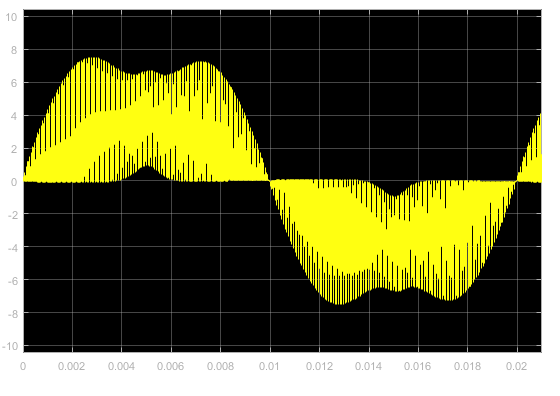
\includegraphics[width=0.82\textwidth]{sonuclar/eski_sekil_4_29_sin3_l1.png}
  \caption{Sin\textsuperscript{3} kompanzasyonlu nötr susturma benzetiminde $L_1$ akımının büyütülmüş görünümü (Senaryo~3).}
  \label{fig:sin3-l1-yakin}
\end{figure}

\begin{figure}[H]
  \centering
  \includegraphics[width=0.98\textwidth]{../dosyalar/05_sonradan_gelenler/Senaryo_3/dalga_sekilleri_s3.jpg}
  \caption{Sin\textsuperscript{3} kompanzasyonlu yöntemde filtre girişi gerilimi, filtrelenmiş gerilim, $L_1$ akımı ve çıkış akımı (Senaryo~3).}
  \label{fig:sin3-dort-kanal}
\end{figure}

Şekil~\ref{fig:sin3-dort-kanal} altında, susturma yönteminin Şekil~\ref{fig:susturma-dort-kanal} üzerindeki belirgin zarf bozulması kompanzasyon sonrasında azalmıştır; ancak çıkış akımı klasik yöntemdeki kadar sinüzoidal hâle gelmemiştir. Görsel karşılaştırma, aynı analiz penceresindeki FFT değerleriyle birlikte okunmalıdır.

\begin{figure}[H]
  \centering
  \includegraphics[width=0.98\textwidth]{../dosyalar/05_sonradan_gelenler/Senaryo_3/THD_IL1.jpg}
  \caption{Sin\textsuperscript{3} kompanzasyonlu yöntemde $L_1$ akımı FFT sonucu: temel bileşen \SI{3.752}{\ampere}, $\mathrm{THD}_{L1}=\%9{,}46$ (Senaryo~3).}
  \label{fig:sin3-l1-fft}
\end{figure}

\begin{figure}[H]
  \centering
  \includegraphics[width=0.98\textwidth]{../dosyalar/05_sonradan_gelenler/Senaryo_3/THD_Iout.jpg}
  \caption{Sin\textsuperscript{3} kompanzasyonlu yöntemde çıkış akımı FFT sonucu: temel bileşen \SI{3.766}{\ampere}, $\mathrm{THD}_{\mathrm{out}}=\%7{,}79$ (Senaryo~3).}
  \label{fig:sin3-iout-fft}
\end{figure}

Senaryo~3'te $L_1$ THD değeri susturma durumundaki \%46,86'dan \%9,46'ya, çıkış THD değeri ise \%46,35'ten \%7,79'a düşmüştür. İyileşme, Sin\textsuperscript{3} yolunun üçüncü harmonik cezasını önemli ölçüde azalttığını destekler. Klasik çıkış THD değerinin \%2,14 olması, kompanzasyonlu yöntemin harmonik bakımından klasik yöntemi geçmediğini de açıkça gösterir. Raporlanan \%93,70 verim değeri, ham kayıp modeli mevcut olmadığından yeniden doğrulanmış bir sonuç değildir.

Düşük, orta ve nominal güçte aynı denetim yapısının karşılaştırılması henüz tamamlanmış bir sonuç seti değildir; mevcut arşiv yalnız düşük güç kayıtlarını içermektedir. Tablo~\ref{tab:sin3-guc-karsilastirma-plani}, gelecek gerçek veri setinde doldurulacak ortak değerlendirme biçimini kilitlemektedir.

\begin{table}[htbp]
  \centering
  \caption{Sin\textsuperscript{3} kompanzasyonu için güç seviyesine bağlı ortak karşılaştırma tablosu.}
  \label{tab:sin3-guc-karsilastirma-plani}
  \small
  \begin{tabularx}{\textwidth}{p{0.14\textwidth} p{0.17\textwidth} X X}
    \toprule
    Güç bölgesi & Karşılaştırma kolları & Ölçülecek kararlı durum büyüklükleri & Geçici durum ve sınır kontrolleri \\
    \midrule
    Düşük & Klasik; susturma; susturma + Sin\textsuperscript{3} & Verim, $I_1$, THD, $I_3/I_1$, ters akım alanı, RMS akım & Kip geçişi, sıfır geçişi, minimum darbe, doyum \\
    Orta & Aynı üç kol & Aynı metrikler ve aynı FFT penceresi & Kompanzasyonun yumuşak azaltılması, akım basamağı \\
    Nominal & Klasik ve nihai öneri; güvenliyse üç kol & Verim, THD, sıcaklık, DA bara dengesi, güç faktörü & Akım sınırı, modülasyon doyumu, koruma ve toparlanma \\
    \bottomrule
  \end{tabularx}
\end{table}

\subsection{Bağımsız Yeniden Üretim Koşuları}

Eldeki dosya paketi Senaryo~1'e ait tek bir kaynak model ve Senaryo~1--3 için özet değerler içeren bir çalışma kitabı sağlamaktadır; Senaryo~2 ve Senaryo~3'e ait kaynak model ya da ham zaman serisi mevcut değildir. Senaryo~1 modeli R2023b ile kaydedilmiştir ve R2025b'de kaldırılan Specialized Power Systems ölçüm bloklarını içerdiği için değişmeden koşturulamamıştır. R2025b çalışma kopyasında $L_1$--$C_f$--$L_2$ değerleri \SI{600}{\micro\henry}--\SI{8}{\micro\farad}--\SI{200}{\micro\henry} yapılmış; dış IGBT'ler SKM100GB12T4, iç IGBT'ler IXYN100N65C3H1 ve yalnız harici iki diyot DSEI2x61-12B olarak eşlenmiştir.

Tablo~\ref{tab:r2025b-senaryo1-dogrulama}, çalışma kopyasıyla yapılan kademeli koşuları ayırmaktadır. Tam cihaz dinamikli \SI{1}{\milli\second} sağlık kontrolü başarıyla tamamlanmış, böylece blok eşlemesi ve elektriksel çözümün R2025b'de ilerlediği doğrulanmıştır. Aynı katmanda \SI{5}{\milli\second} koşu 1200~s duvar süresi içinde tamamlanmadığından hesap maliyeti sınırıyla sonlandırılmış, sayısal başarısızlık olarak etiketlenmemiştir. Cihaz dinamikleri sadeleştirilen \SI{25}{\milli\second} sistem koşusu ise \SI{21.3324}{\milli\second} anında diyot denklemlerinin yakınsamamasıyla durmuştur. Tam bir \SI{50}{\hertz} kararlı hâl penceresi ve geçerli THD/verim sonucu bu yüzden oluşmamıştır.

\begin{table}[htbp]
  \centering
  \caption{Seçilen LCL ve yarıiletken eşlemesiyle R2025b Senaryo~1 kademeli doğrulama koşuları.}
  \label{tab:r2025b-senaryo1-dogrulama}
  \footnotesize
  \begin{tabularx}{\textwidth}{>{\raggedright\arraybackslash}p{0.19\textwidth} >{\raggedright\arraybackslash}p{0.16\textwidth} >{\raggedright\arraybackslash}p{0.20\textwidth} >{\raggedright\arraybackslash}X}
    \toprule
    Koşu & Ufuk & Sonuç & Kanıt sınırı \\
    \midrule
    Seçilen filtre, sade sistem & \SI{5}{\milli\second} & Başarılı; son \%20 pencerede $I_{\mathrm{ac,rms}}=\SI{2.428}{\ampere}$ & Kısa süreli fiziksel tutarlılık; THD/verim değil. \\
    Seçilen filtre ve doğrulanmış cihazlar & \SI{1}{\milli\second} & Başarılı; 26,7~s hesap süresi & Cihaz/blok sağlık kontrolü; başlangıç geçicisi baskın. \\
    Aynı ayrıntılı cihaz katmanı & \SI{5}{\milli\second} & 1200~s içinde tamamlanmadı & Hesap maliyeti sınırı; performans sonucu yok. \\
    Seçilen filtre, sade sistem & \SI{25}{\milli\second} & \SI{21.3324}{\milli\second}'de yakınsama hatası & Kararlı hâl, THD ve verim geçersiz. \\
    \bottomrule
  \end{tabularx}
\end{table}

\SI{1}{\milli\second} koşuda ham DA bara gerilimi \SI{431.5}{\volt} olarak korunurken ideal gerilim kaynağının boş DA-link kapasitörlerini aniden şarj etmesi \SI{43.1}{\kilo\ampere} düzeyinde fiziksel olmayan bir başlangıç tepesi oluşturmuştur. Bu ilk koşul giderilmeden ve en az iki kararlı temel periyot tamamlanmadan ekrandaki anık güç, THD ve verim değerleri kullanılmamıştır; çalışma kitabında bildirilen \%92,5 verim ve yaklaşık \%15 THD, yeniden üretilmiş sonuç değil deney özeti olarak tutulmuştur.

Topoloji ve kapı mantığı bakımından bağımsız kontrol amacıyla, 12 IGBT'li üç fazlı Simscape modeli aynı koşullarda koşturulmuştur. Modelde klasik, nötr susturma ve susturma+$K_{\mathrm{sin3}}=-\SI{2}{\volt}$ kolları için geçersiz anahtarlama durumu sayısı sıfırdır; Tablo~\ref{tab:yeniden-uretim-fiziksel-s123} sonuçları vermektedir. Geçici model değerleri ($V_{\mathrm{dc}}=\SI{400}{\volt}$, $L_1=\SI{2}{\milli\henry}$, $L_2=\SI{1}{\milli\henry}$ ve \SI{2}{\micro\second} deneme ölü zamanı) kaynak modelle aynı olmadığından koşu bir parça-kayıp veya verim doğrulaması değildir.

\begin{table}[htbp]
  \centering
  \caption{Üç fazlı fiziksel model koşusu (22.08.2026); kaynak Senaryo~1--3'ün sayısal yeniden üretimi değil, kapı durumu ve yöntem yönelimi kontrolüdür.}
  \label{tab:yeniden-uretim-fiziksel-s123}
  \small
  \begin{tabularx}{\textwidth}{X r r r r}
    \toprule
    Yöntem & Faz RMS (A) & Ortalama THD (\%) & Nötr RMS (A) & Geçersiz durum \\
    \midrule
    Klasik & 2,227 & 10,898 & 0,639 & 0 \\
    Nötr susturma & 2,238 & 13,625 & 0,711 & 0 \\
    Susturma+Sin\textsuperscript{3} & 2,209 & 13,772 & 0,694 & 0 \\
    \bottomrule
  \end{tabularx}
\end{table}

Bu yeniden koşuda Sin\textsuperscript{3} terimi nötr RMS akımını yalnız susturmaya göre yaklaşık \%2,46 azaltmış, fakat faz THD'sini iyileştirmemiştir. Sonucun Senaryo~3 eğilimini yeniden üretmemesi bir başarısızlık gizleme nedeni değil, enjeksiyon noktası ile $K_1/K_3$ ölçeklerinin gerçek koddan kilitlenmesi gerektiğini gösteren negatif doğrulamadır; Kesim~\ref{sec:sin3-yeniden-tarama} altındaki katsayı taşınamazlığı bulgusuyla da tutarlıdır. Şekil~\ref{fig:yeniden-uretim-fiziksel-s123} kullanılan kazanç noktalarını ve iki metriği birlikte göstermektedir.

\begin{figure}[htbp]
  \centering
  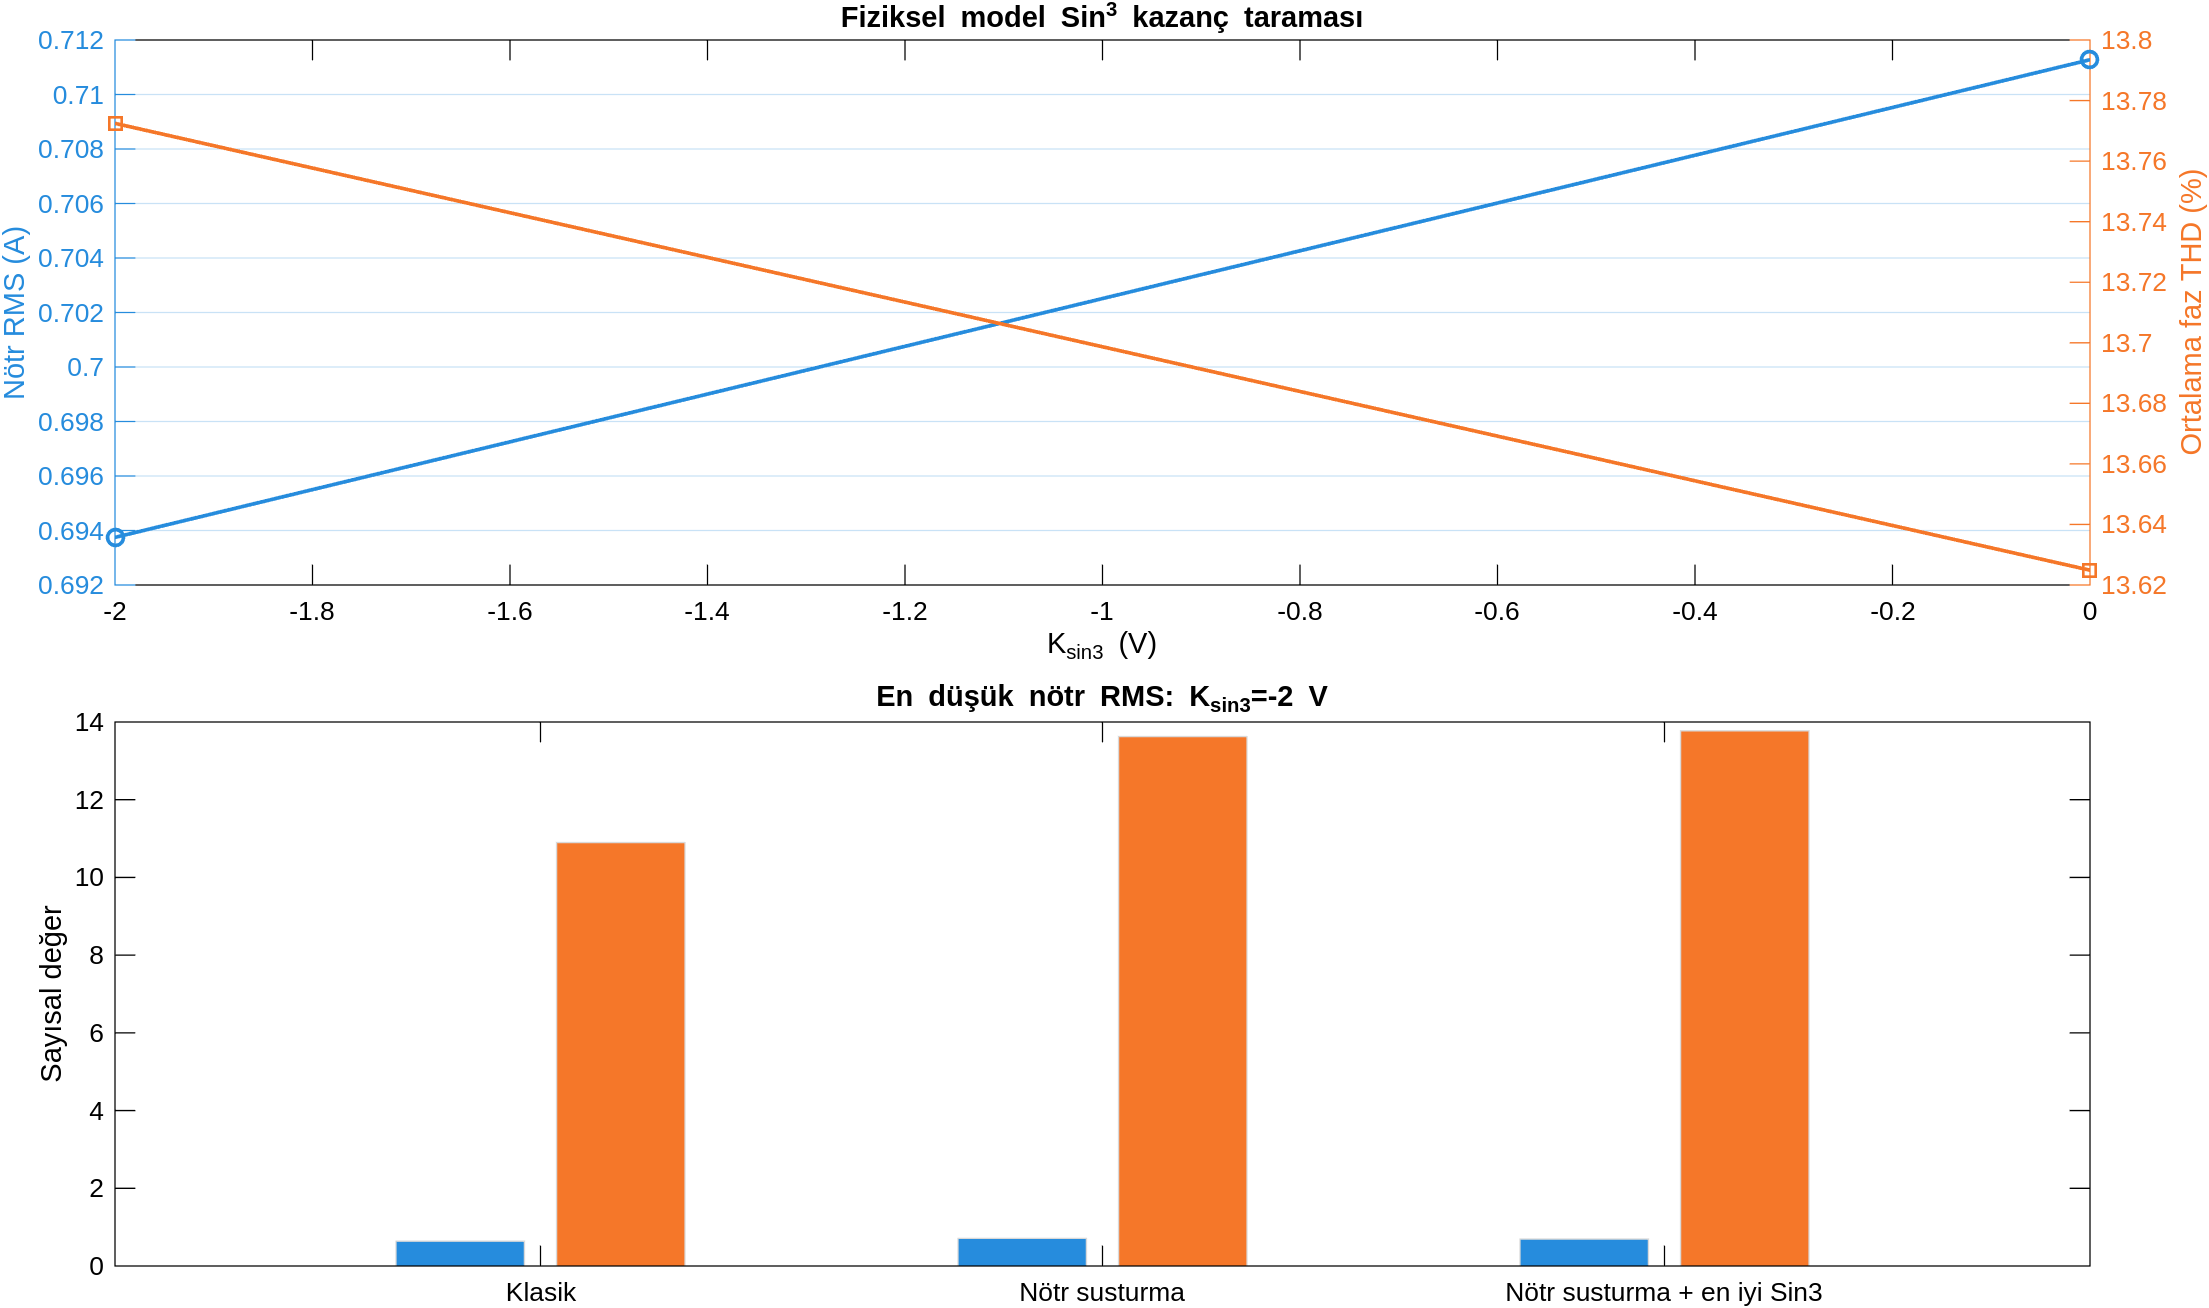
\includegraphics[width=0.96\textwidth]{sonuclar/fiziksel_senaryo123_20260822.png}
  \caption{Üç fazlı fiziksel yeniden koşuda nötr RMS ve ortalama faz THD karşılaştırması. Sonuçlar geçici fiziksel model parametreleriyle sınırlıdır.}
  \label{fig:yeniden-uretim-fiziksel-s123}
\end{figure}

Senaryo~4 için ayrıca, verilen $L_1=\SI{600}{\micro\henry}$, $R_1=\SI{0.02}{\ohm}$, $V_{\mathrm{dc}}=\SI{431}{\volt}$ ve \SI{120}{\volt} RMS şebeke değerleriyle ortalama-değerli bir akım-döngüsü fizibilite deneyi yapılmıştır. İleri besleme $K_1\sin(\theta+\phi)+K_3\sin^3(\theta)$ biçiminde, geri besleme ise $L_1$ akımıyla çalışan PI çıkışı olarak aynı gerilim komutunda toplanmıştır. Hedef ``30~A'' ifadesi tepe mi RMS mi belirtmediğinden iki yorum da sınanmıştır. PI kazançları $K_p=\SI{3}{\volt\per\ampere}$ ve $K_i=\SI{100}{\volt\per\ampere\second}$, denetim periyodu \SI{100}{\micro\second} ve $K_3=-\SI{2}{\volt}$ seçilmiştir.

\begin{table}[htbp]
  \centering
  \caption{Senaryo~4 ortalama-değerli PI fizibilite deneyi; yarı iletken anahtarlama kaybı ve verim kapsam dışıdır.}
  \label{tab:senaryo4-pi-30a}
  \small
  \begin{tabularx}{\textwidth}{p{0.17\textwidth} X r r r r}
    \toprule
    30 A yorumu & Denetim & Ölçülen RMS (A) & RMSE (A) & THD (\%) & $|m|_{\max}$ \\
    \midrule
    Tepe (21,213 A RMS) & İleri besleme & 11,742 & 11,187 & 5,326 & 0,781 \\
    Tepe (21,213 A RMS) & İleri besleme+PI & 20,922 & 0,665 & 0,559 & 0,791 \\
    RMS & İleri besleme & 20,138 & 11,135 & 3,103 & 0,783 \\
    RMS & İleri besleme+PI & 29,715 & 0,662 & 0,393 & 0,793 \\
    \bottomrule
  \end{tabularx}
\end{table}

Her iki PI koşusunda da modülasyon doyumu oluşmamış ve referans izleme belirgin biçimde iyileşmiştir. Şekil~\ref{fig:senaryo4-pi-30a}, son iki periyottaki akımları ve modülasyon payını göstermektedir. Sonuç, yaklaşık 30~A akımın ileri besleme+PI yapısıyla ortalama modelde izlenebildiğini kanıtlar; anahtarlamalı LCL model, cihaz kayıpları, termal portlar ve gerçek PI kodu eklenmeden verim veya donanım kararlılığı iddiası kurmaz.

\begin{figure}[htbp]
  \centering
  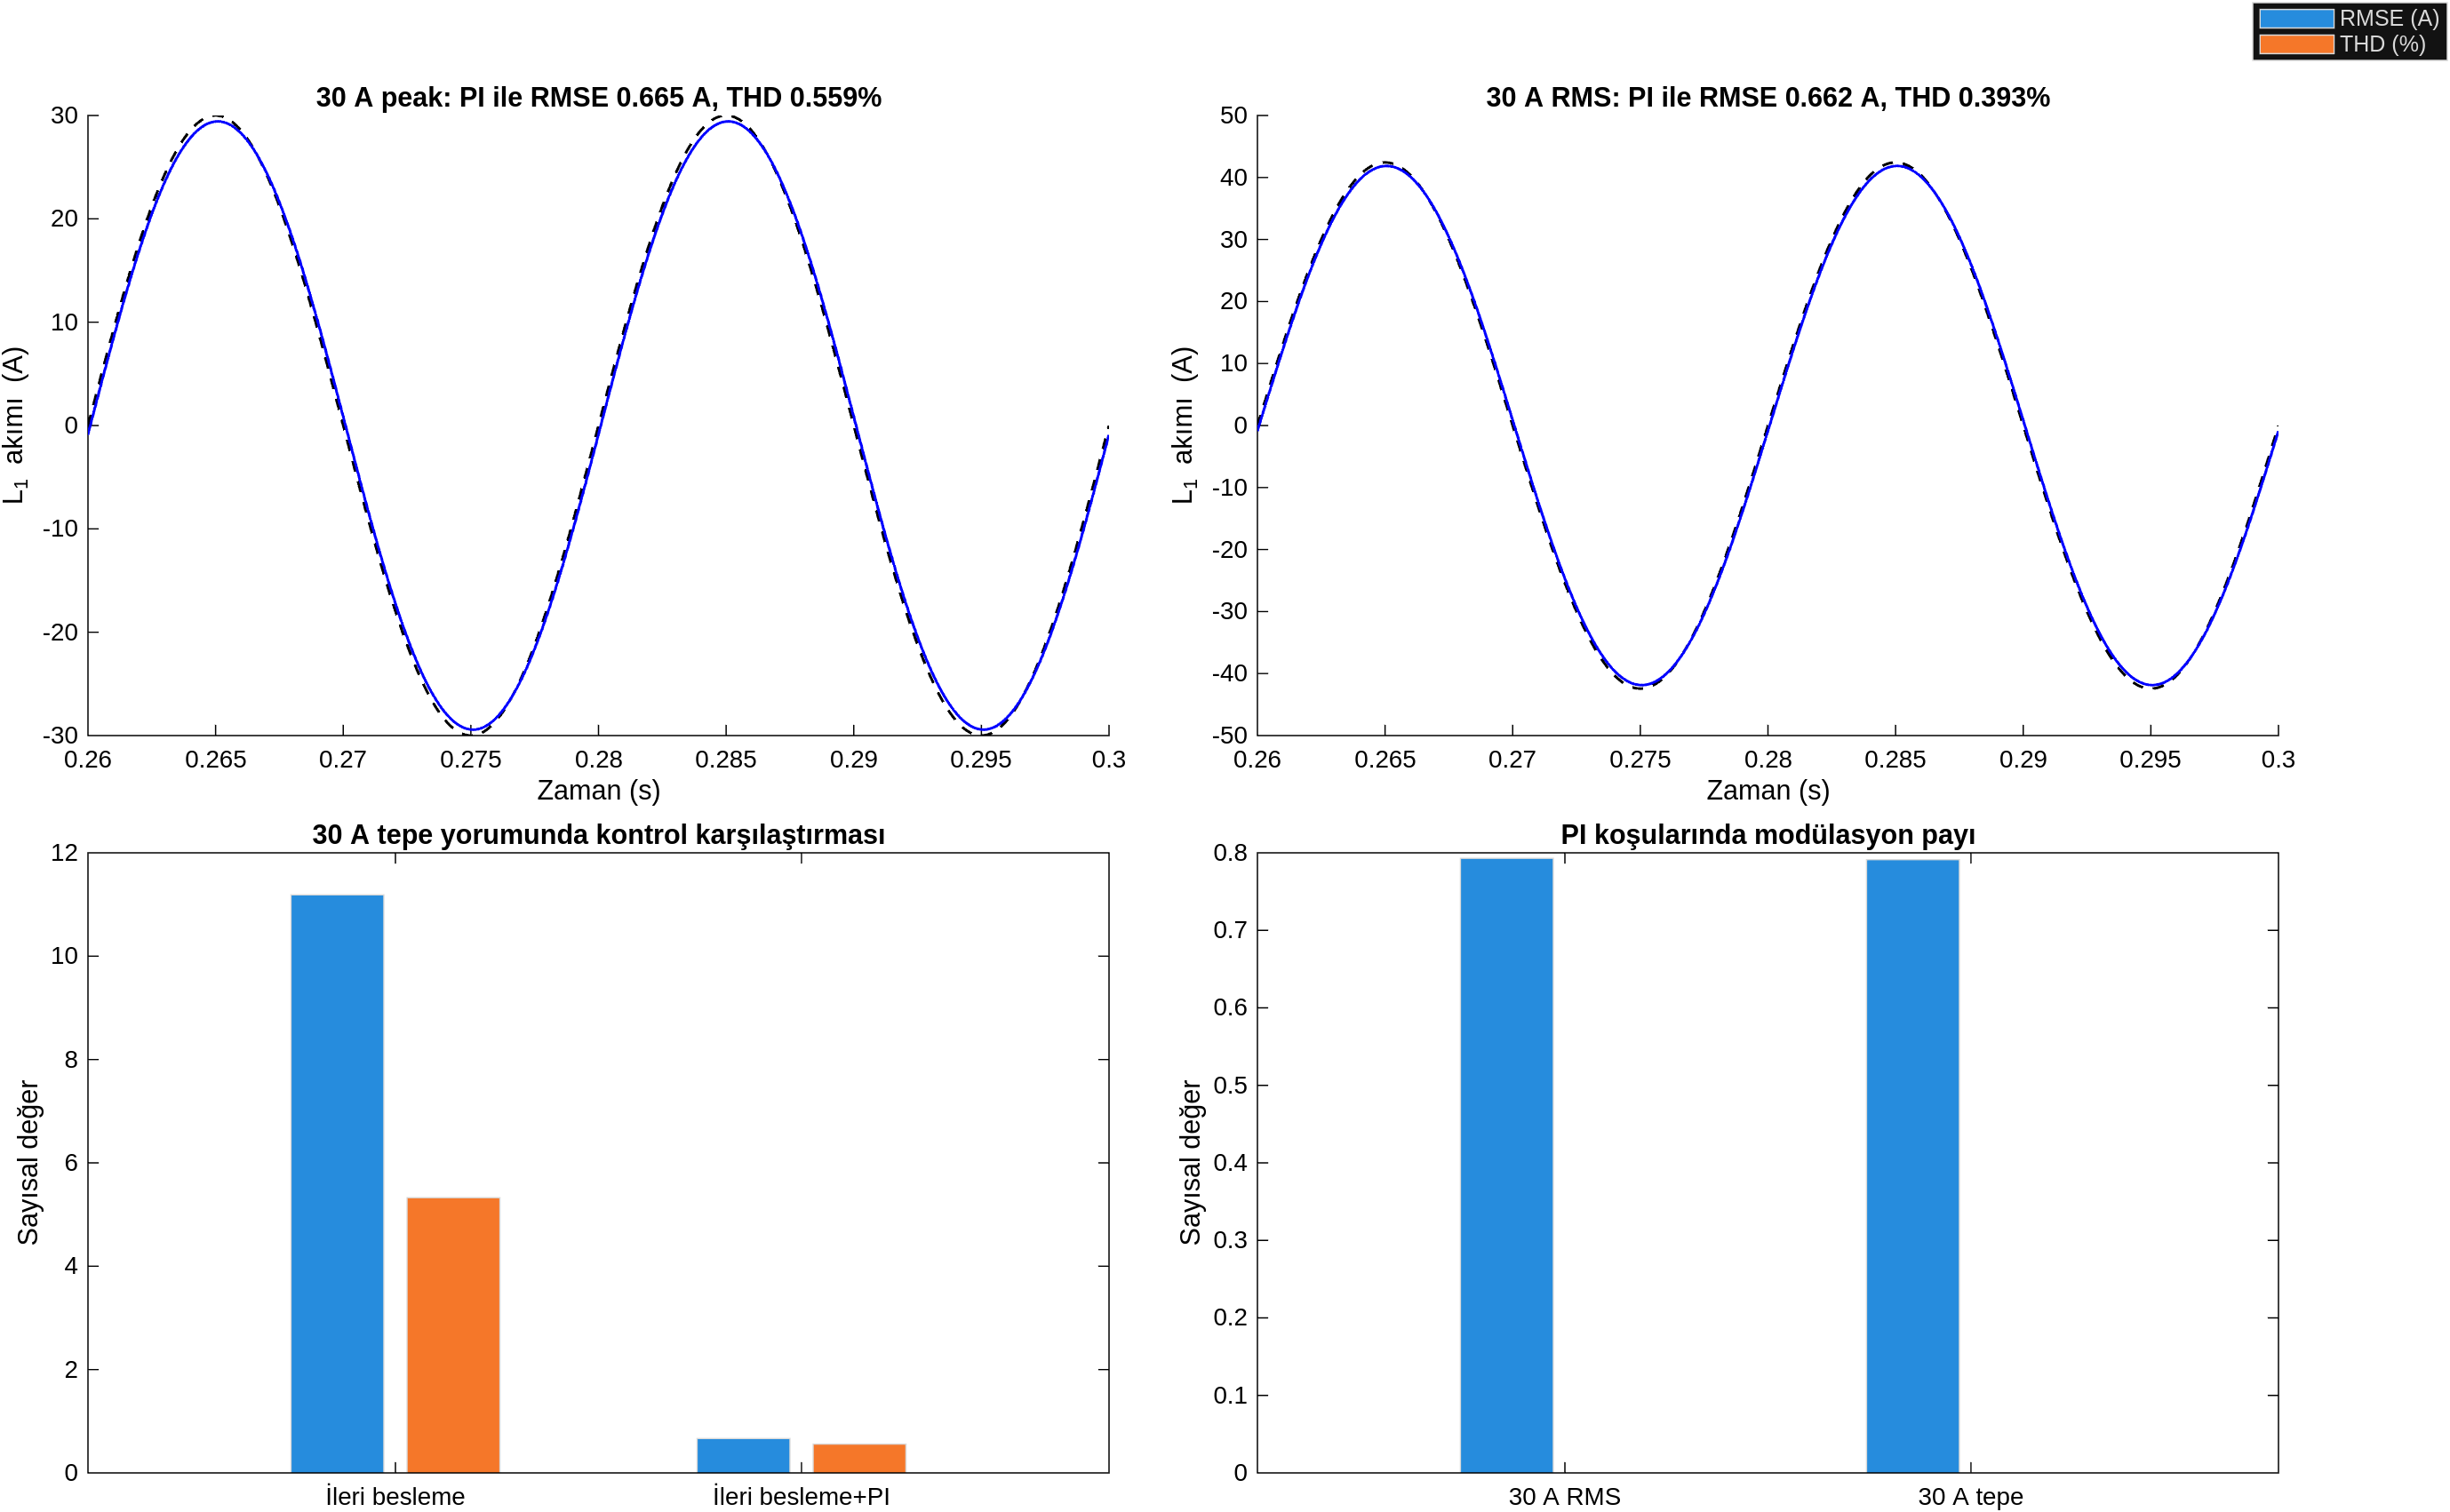
\includegraphics[width=0.98\textwidth]{sonuclar/senaryo4_pi_30a_20260822.png}
  \caption{Senaryo~4 için 30~A tepe ve 30~A RMS yorumlarında ileri besleme+PI akım izleme fizibilitesi ve modülasyon payı.}
  \label{fig:senaryo4-pi-30a}
\end{figure}

Nihai kazanç seçimi düşük güçte tek bir THD minimumuna göre yapılmayacaktır. Aday kazançlar önce düşük güçte ters akım--THD ödünleşimiyle taranacak, ardından orta ve nominal güçte kompanzasyonun gereksiz temel bileşen değişimi veya doyum üretmediği doğrulanacaktır. Aynı denetleyici katsayılarının bütün güç aralığında korunması hedeflenecek; kazanç çizelgelemesi gerekirse etkinleştirme eşiği, histerezis ve geçiş sürekliliği açıkça raporlanacaktır.

\section{Bölüm Sonucu}

Sin\textsuperscript{3} özdeşliği temel ve üçüncü harmonik bileşenini tek bir anlık terimde birleştirmekte, ancak doğrudan $\sin(3\theta)$ enjeksiyonuyla aynı katsayı anlamını taşımamaktadır. DCM/CCM parçalı modeli, nötr susturma sonrasında sinüzoidal görev oranının neden sinüzoidal akım üretmediğini göstermiş; doğru özdeşlikle yapılan katsayı taraması saf sinüs görev oranındaki \%39,96'lık üçüncü harmonik oranını, doğrulanmış parametre setiyle uyumlu $(D_1,D_3)=(0{,}34,\ 0{,}40)$ noktasında \%0,15'e indiren düzeltilmiş bir aday üretmiştir. Aynı tarama, önceki aday katsayıların bu parametre setine taşınamadığını sayısal olarak göstermiştir; katsayı seçimi çalışma noktasına bağlıdır.

Kapalı çevrim yapı Sin\textsuperscript{3} terimini bağımsız kontrolcü olarak değil, akım döngüsünün modülasyon toplamına eklenen ileri besleme girişi olarak konumlandırmıştır. Geçici MATLAB modeli $L$, $S$ ve $T$ analiz zincirini ve şebeke endüktansı taramasını çalıştırmaktadır; sayısal kararlılık marjları gerçek parametre doğrulaması beklemektedir. Bağımsız fiziksel koşu tarihsel THD iyileşmesini yeniden üretmemiş ve gerçek enjeksiyon/kazanç eşleşmesinin zorunluluğunu göstermiştir. Senaryo~4 ortalama modeli, yaklaşık 30~A akımın PI ile doyumsuz izlenebildiğini göstermiştir; orta ve nominal güçte anahtarlamalı verim, termal durum, THD ve geçici rejim karşılaştırması gerçek model ve ölçüm verileriyle tamamlanmalıdır.
